\clearpage
\section{Diseño}

\subsection{Requisitos del sistema y especificación técnica}

A partir de los objetivos específicos planteados en el Capítulo~1 (OE1 a OE6) y del protocolo experimental establecido en el Capítulo~3, se formalizan los requisitos funcionales y no funcionales que rigen la arquitectura del sistema de generación e inspección de campos de distancia con signo (SDF) en GPU. La Tabla~\ref{tab:requisitos_sistema} sintetiza la especificación de requisitos y su trazabilidad con los objetivos del trabajo.

\begin{table}[htbp]
  \centering
  \footnotesize
  \caption{Especificación de requisitos funcionales y no funcionales del sistema.}
  \label{tab:requisitos_sistema}
  \begin{tabularx}{\textwidth}{|>{\bfseries}c|>{\bfseries\raggedright\arraybackslash}p{31mm}|c|>{\raggedright\arraybackslash}X|}
    \hline
    \rowcolor{tablegray} ID & Categoría & Objetivo & Descripción del requisito \\ \hline
    RF1 & Importación y preprocesamiento geométrico & OE3, OE4 & Cargar mallas poligonales en formatos glTF 2.0 y GLB, aplanar su jerarquía de transformaciones, soldar vértices coincidentes, calcular pseudo-normales ponderadas por ángulo y empaquetar las primitivas en un \textit{buffer} SSBO (\texttt{std430}). \\ \hline
    RF2 & Generación exacta de referencia en GPU & OE3 & Calcular en GPU la distancia euclídea mínima punto-triángulo sobre los $V^3$ vóxeles utilizando memoria compartida por bloque y determinación del signo mediante ángulos sólidos (\textit{Generalized Winding Numbers}). \\ \hline
    RF3 & Generación acelerada mediante JFA 3D & OE4 & Generar volúmenes SDF mediante propagación JFA 3D ($\mathcal{O}(V^3 \log_2 V)$) con tres variantes de salto ($\text{JFA}$, $\text{JFA}+1$ y $1+\text{JFA}$) y tres modalidades de captura de semillas: voxelización de corteza, atlas G-Buffer ortográfico de 6 vistas y G-Buffer de cámara. \\ \hline
    RF4 & Determinación del signo y superficies abiertas & OE3, OE4 & Soportar tanto el cálculo de signo exacto en mallas cerradas (votación de arrollamiento en 6 direcciones axiales y respaldo de normal local) como distancias sin signo y láminas de doble cara (\textit{double-sided}) en escenas abiertas. \\ \hline
    RF5 & Trazado volumétrico y objetos dinámicos & OE2 & Integrar el muestreo trilineal de volúmenes SDF estáticos y dinámicos en el \textit{path tracer} a 1 SPP con detección de cruce de signo por bisección, acumulación de semillas en coordenadas locales del objeto móvil y reproyección temporal en SVGF. \\ \hline
    RF6 & Inspección por cortes 2D y métricas GPU & OE5, OE6 & Incorporar un inspector interactivo de cortes ortogonales 2D (isolíneas de distancia/signo y mapa de calor de error absoluto $|f_{\text{JFA}} - f_{\text{ref}}|$) junto con mediciones de tiempos GPU por etapa, VRAM y error (MAE, RMSE, $E_{\max}$ y acuerdo de signo). \\ \hline
    RNF1 & Independencia de hardware propietario & OE1--OE6 & Ejecutar íntegramente sobre el perfil Core de OpenGL 4.6 y \textit{compute shaders} estándar sin depender de núcleos dedicados de trazado de rayos por hardware. \\ \hline
    RNF2 & Parametrización de precisión y memoria & OE3, OE4, OE6 & Admitir formatos volumétricos de 32 bits (\texttt{GL\_R32F}) y 16 bits (\texttt{GL\_R16F}) en resoluciones desde $24^3$ hasta $256^3$ vóxeles, reutilizando los recursos temporales asignados en VRAM. \\ \hline
    RNF3 & Desacoplamiento de tiempos de medición & OE5, OE6 & Separar mediante consultas asíncronas en hardware (\texttt{GL\_TIMESTAMP} y \texttt{GL\_TIME\_ELAPSED}) el coste de construcción del SDF respecto al tiempo de renderizado y trazado de caminos. \\ \hline
    RNF4 & Verificabilidad y pruebas de regresión & OE1--OE6 & Disponer de una batería automatizada de pruebas en GPU (\texttt{render\_tests}) que verifique sin intervención manual la exactitud del campo, la ausencia de \texttt{NaN}/\texttt{Inf}, la convergencia temporal y las sombras dinámicas. \\ \hline
  \end{tabularx}
\end{table}

\subsection{Arquitectura global del software e inventario de recursos}

El sistema se ha diseñado siguiendo una arquitectura modular en C++20 desacoplada en cuatro subsistemas principales: el núcleo de aplicación e interfaz diagnóstica, el subsistema de importación y preparación geométrica, el motor de generación y comparación de volúmenes SDF en GPU, y la canalización de renderizado por trazado de caminos con reconstrucción espacio-temporal. Tal como muestra la Figura~\ref{fig:arquitectura_componentes}, la comunicación entre los módulos de CPU y los procesos masivamente paralelos en GPU se articula a través de objetos de almacenamiento \texttt{std430} (\textit{Shader Storage Buffer Objects}, SSBO), texturas volumétricas tridimensionales (\texttt{GL\_TEXTURE\_3D}) vinculadas mediante unidades de imagen (\texttt{image3D} / \texttt{uimage3D} / \texttt{iimage3D}) y objetivos de renderizado múltiple (\textit{Multiple Render Targets}, MRT).

\begin{figure}[htbp]
  \centering
  \begin{tikzpicture}[
    node distance=6mm and 6mm,
    font=\footnotesize\sffamily,
    box/.style={draw=black, line width=0.6pt, rounded corners=2pt, align=center, inner sep=4pt},
    appbox/.style={box, fill=uocblue!10, text width=140mm, line width=0.8pt},
    modbox/.style={box, fill=white, text width=66mm, line width=0.8pt},
    gpubox/.style={box, fill=uoccyan!18, text width=42mm},
    resbox/.style={box, fill=tablegray, text width=66mm},
    arr/.style={->, >=Latex, line width=0.75pt}
  ]
    % Top Application Layer
    \node[appbox] (app) {\textbf{Application Layer (\texttt{main.cpp}, \texttt{Scenes.h}, Dear ImGui UI)}\\Scene Manager, Parameter Controls, Live GPU Profiler, Automated Regression Runner};

    % Middle CPU Modules
    \node[modbox, anchor=north west] (model) at ([yshift=-6mm]app.south west) {\textbf{Mesh Processor (\texttt{renderer::Model})}\\glTF 2.0 / GLB Loader, Hierarchy Flattener,\\Vertex Welder, Angle-Weighted Normals};
    \node[modbox, anchor=north east] (gen) at ([yshift=-6mm]app.south east) {\textbf{SDF Engine (\texttt{renderer::SdfGenerator})}\\Exact Baseline Dispatcher, 3D JFA Pipeline,\\6-Axis Winding Sign, Error Metrics Evaluator};

    % GPU Compute Resources
    \node[resbox, below=6mm of model] (ssbo) {\textbf{GPU Geometry Buffers}\\Packed \texttt{GpuTriangle} SSBO (\texttt{std430}, 96 B/tri)\\+ 6-View Orthographic \& Camera G-Buffer FBOs};
    \node[resbox, below=6mm of gen] (vol) {\textbf{3D Volume Textures (\texttt{Texture3D})}\\Static Scene SDF + Dynamic Local SDF (\texttt{R32F}/\texttt{R16F})\\Seed Ping-Pong (\texttt{RGBA32F}) \& Atomic Grids (\texttt{R32UI})};

    % Bottom Rendering & Inspection Pipeline
    \node[appbox, fill=white, anchor=north west] (pipe) at ([yshift=-6mm]ssbo.south west) {\textbf{Rendering and Inspection Pipeline (\texttt{renderer::PathTracerPipeline})}\\Primary G-Buffer Pass $\rightarrow$ 1-SPP SDF Sphere Tracer $\rightarrow$ SVGF Temporal \& À-Trous Filter $\rightarrow$ 2D Slice Inspector \& FXAA};

    % GPU Shaders bottom row
    \node[gpubox, anchor=north west] (sh1) at ([yshift=-6mm]pipe.south west) {\textbf{Compute Shaders}\\Exact Baseline, Seed Voxelize/Resolve, JFA Step, Winding};
    \node[gpubox, below=6mm of pipe] (sh2) {\textbf{Ray Marching Shader}\\3D SDF Bisection, Dynamic Grid Trace, STBN Sampling};
    \node[gpubox, anchor=north east] (sh3) at ([yshift=-6mm]pipe.south east) {\textbf{Resolve \& Slice Shader}\\SVGF Denoiser, 2D Orthogonal Isolines \& Error Heatmap};

    % Connections
    \draw[arr] (app.south -| model.north) -- (model.north);
    \draw[arr] (app.south -| gen.north) -- (gen.north);
    \draw[arr] (model.east) -- (gen.west);
    \draw[arr] (model.south) -- (ssbo.north);
    \draw[arr] (ssbo.east) -- (gen.south west);
    \draw[arr] (gen.south) -- (vol.north);
    \draw[arr] (ssbo.south) -- (pipe.north -| ssbo.south);
    \draw[arr] (vol.south) -- (pipe.north -| vol.south);
    \draw[arr] (pipe.south -| sh1.north) -- (sh1.north);
    \draw[arr] (pipe.south -| sh2.north) -- (sh2.north);
    \draw[arr] (pipe.south -| sh3.north) -- (sh3.north);
  \end{tikzpicture}
  \caption{Arquitectura modular de componentes en C++20 y flujo de recursos en GPU.}
  \label{fig:arquitectura_componentes}
\end{figure}

De acuerdo con las pautas de documentación técnica y trazabilidad de autoría, la Tabla~\ref{tab:inventario_assets} detalla el inventario completo de activos geométricos, texturas y recursos de software que intervienen en las escenas del proyecto, diferenciando explícitamente los elementos diseñados y programados por el autor de los modelos tridimensionales y máscaras estocásticas reutilizados de terceros.

\begin{table}[htbp]
  \centering
  \small
  \caption{Inventario de activos (\textit{assets}), escenas y recursos técnicos del proyecto.}
  \label{tab:inventario_assets}
  \begin{tabularx}{\textwidth}{|>{\bfseries\raggedright\arraybackslash}p{35mm}|>{\raggedright\arraybackslash}p{26mm}|>{\raggedright\arraybackslash}p{30mm}|>{\raggedright\arraybackslash}X|}
    \hline
    \rowcolor{tablegray} Recurso / Activo & Autoría / Origen & Formato / Especificación & Características técnicas y función en el sistema \\ \hline
    Generadores SDF y canalización de shaders GLSL & Autor (desarrollo propio en el TFM) & 11 \textit{compute shaders} y 10 shaders gráficos (GLSL 4.60) & Implementación íntegra del método base exacto, voxelización atómica de semillas, propagación JFA 3D, barrido axial de signo en 6 direcciones, trazado con bisección e inspector de cortes 2D. \\ \hline
    Geometrías analíticas y escenas CSG (Escenas 1, 2, 3 y 5) & Autor (con funciones base \texttt{hg\_sdf}) & Código GLSL inyectado en tiempo de ejecución & Definición matemática de la caja de Cornell acotada, muestrario de materiales reflexivos, pedestal híbrido con orbes emisivos y estancia cerrada con ventana sustraída mediante diferencia booleana. \\ \hline
    Oclusor dinámico deformable (\texttt{StretchingBox}) & Autor (desarrollo propio en el TFM) & Geometría procedimental en shader (\texttt{stretching\_box.\allowbreak vert}) & Ortoedro animado de extensión biaxial variable y espesor físico parametrizable entre $0,1\text{ mm}$ y $100\text{ mm}$ para estudiar fugas de luz y espesor aparente en volúmenes SDF dinámicos. \\ \hline
    Malla poligonal \textbf{Suzanne} (\texttt{demo.gltf}) & Terceros (Blender Foundation, Dominio Público / GPL) & glTF 2.0 con \textit{buffer} binario codificado en Base64 & Malla de prueba ($968$ triángulos) empleada tanto en generación volumétrica estática (Escenas 1, 3, 4 y 5) como en el experimento de objeto móvil con rotación y persistencia local en Sponza (Escena 6). \\ \hline
    Escena arquitectónica \textbf{Crytek Sponza} (\texttt{sponza.glb}) & Terceros (M. Dabrovic / Crytek / M. McGuire, CC BY 3.0) & Binario glTF 2.0 (\texttt{.glb}) + 69 texturas PNG PBR & Modelo arquitectónico de alta complejidad ($262.267$ triángulos) con múltiples materiales PBR (mapas de albedo sRGB, normales y rugosidad-metalicidad), arcos, columnas y cortinas de doble cara. \\ \hline
    Máscaras de ruido azul \textbf{STBN} (\texttt{stbn0.bin}, \texttt{stbn1.bin}) & Terceros (NVIDIA Research, Wolfe et al. \cite{wolfe2022egsr}) & Texturas 3D binarias \texttt{GL\_RGBA8} ($128\times 128\times 64$) & Secuencias precomputadas \textit{void-and-cluster} de ruido azul espaciotemporal para estratificar el muestreo de Monte Carlo a 1 SPP y suprimir la ebullición de baja frecuencia en SVGF. \\ \hline
  \end{tabularx}
\end{table}

\subsection{Preprocesamiento geométrico y empaquetado de mallas para GPU}

Para alimentar tanto el generador de referencia como las variantes basadas en JFA 3D y el pase de rasterización de materiales, la clase \texttt{renderer::Model} implementa un cargador y preprocesador nativo de archivos glTF 2.0 (\texttt{.gltf}) y contenedores binarios GLB (\texttt{.glb}) apoyado en \texttt{nlohmann/json}. El procesamiento de una malla desde su lectura en disco hasta su transferencia a la memoria de vídeo comprende cuatro etapas deterministas:

\begin{enumerate}
  \item \textbf{Recorrido jerárquico del grafo de escena y extracción de materiales PBR:} El cargador decodifica los \textit{buffers} binarios (archivos externos, bloques \texttt{BIN} de GLB o cadenas URI en Base64) y recorre recursivamente el árbol de nodos aplicando las transformaciones locales (matrices $4\times 4$ o composición de traslación, cuaternión de rotación y escala). Por cada primitiva geométrica se registran su rango de índices (\texttt{PrimitiveRange}) y sus propiedades de material glTF 2.0 \cite{khronos_gltf2}: factor de color base, rugosidad, metalicidad, escala de normal, umbral de recorte alfa (\texttt{alphaCutoff}), atributo de doble cara (\texttt{doubleSided}) e identificadores de texturas asociadas.
  \item \textbf{Normalización espacial y ajuste automático al volumen (\texttt{computeFitTransform}):} Durante la extracción de vértices se calcula la caja delimitadora alineada con los ejes (\textit{Axis-Aligned Bounding Box}, AABB) del modelo completo, definida por $\text{AABB}_{\min}$ y $\text{AABB}_{\max}$. Dado un volumen SDF cúbico de tamaño métrico $W$ (\texttt{worldSize}) centrado en $\mathbf{o}_w$ (\texttt{worldOffset}) y una fracción de margen de guarda $\rho \in [0, 1)$ ($0,15$ por defecto en volúmenes estáticos y $0,33$ en el volumen dinámico local), se construye una matriz de transformación uniforme que centra y escala isotrópicamente la malla:
  \begin{equation}
    s = \frac{W \cdot (1 - \rho)}{\max\left(\Delta_x, \Delta_y, \Delta_z, 10^{-5}\right)}, \quad \text{con } (\Delta_x, \Delta_y, \Delta_z) = \text{AABB}_{\max} - \text{AABB}_{\min}
  \end{equation}
  \begin{equation}
    \mathbf{M}_{\text{fit}} = \mathbf{T}(\mathbf{o}_w) \cdot \mathbf{S}(s, s, s) \cdot \mathbf{T}\!\left(-\frac{\text{AABB}_{\min} + \text{AABB}_{\max}}{2}\right)
  \end{equation}
  Este margen perimetral garantiza que la isosuperficie cero quede completamente contenida en el interior del dominio discretizado y evita discontinuidades de borde durante el muestreo trilineal.
  \item \textbf{Soldadura espacial de vértices (\textit{vertex welding}) y pseudo-normales ponderadas por ángulo:} Los archivos glTF suelen duplicar vértices a lo largo de las costuras de coordenadas de textura (UV) o límites de grupos de suavizado. Si las normales de vértice se promediaran únicamente por índice de vértice del archivo, las aristas con costuras UV presentarían normales discontinuas que provocarían inversiones de signo en las regiones de Voronoi de arista y vértice \cite{baerentzen2005}. Para resolver este problema, el preprocesador cuantiza las posiciones tridimensionales transformadas sobre una rejilla fina de paso $\epsilon_w = 10^{-5} \cdot \max(\|\text{AABB}_{\max} - \text{AABB}_{\min}\|, 10^{-4})$ e indexa cada posición en una tabla hash espacial (\texttt{WeldKey}). Sobre cada clase de equivalencia geométrica soldada, se acumula la normal de cada cara adyacente $n_{F_k}$ ponderada por el ángulo interior de apertura $\theta_k$ en dicho vértice:
  \begin{equation}
    \theta_k = \arccos\!\left(\text{clamp}\!\left(\frac{\mathbf{e}_{k,1} \cdot \mathbf{e}_{k,2}}{\|\mathbf{e}_{k,1}\| \, \|\mathbf{e}_{k,2}\|}, -1, 1\right)\right), \quad \mathbf{n}_v = \frac{\sum_{k} \theta_k \, \mathbf{n}_{F_k}}{\left\|\sum_{k} \theta_k \, \mathbf{n}_{F_k}\right\|}
  \end{equation}
  Adicionalmente, cuando una primitiva pertenece a un material marcado como de doble cara (\texttt{double\allowbreak Sided}) en glTF (como las cortinas y estandartes de Crytek Sponza), dicho indicador booleano se codifica en la cuarta componente ($w = 1,0$) de los vectores normales del triángulo para que los generadores volumétricos excluyan las láminas abiertas del cálculo de arrollamiento interior/exterior.
  \item \textbf{Empaquetado en \texttt{GpuTriangle} (\texttt{std430}) y caché de validación del SSBO:} Cada triángulo transformado al espacio de mundo se empaqueta en una estructura contigua de 96 bytes compuesta por seis vectores de cuatro componentes en coma flotante de 32 bits, cuya disposición exacta se muestra en la Tabla~\ref{tab:gputriangle_layout}. El motor \texttt{SdfGenerator} mantiene una caché de estado sobre el \textit{buffer} \texttt{m\_triangleSsbo} (número de triángulos, extremos del AABB y matriz de transformación), evitando reconstruir y retransmitir los datos por el bus PCIe cuando se modifican únicamente parámetros del algoritmo como la resolución del volumen o la variante de JFA.
\end{enumerate}

\begin{table}[htbp]
  \centering
  \small
  \caption{Estructura de memoria de \texttt{GpuTriangle} (96 bytes) alineada según el estándar \texttt{std430}.}
  \label{tab:gputriangle_layout}
  \begin{tabularx}{\textwidth}{|>{\bfseries}l|c|c|>{\raggedright\arraybackslash}X|}
    \hline
    \rowcolor{tablegray} Campo & Tipo GLSL / C++ & Offset (Bytes) & Contenido semántico \\ \hline
    \texttt{v0} & \texttt{vec4} / \texttt{glm::vec4} & 0 -- 15 & \texttt{xyz}: posición en mundo del vértice 0; \texttt{w}: reservado ($0,0$). \\ \hline
    \texttt{v1} & \texttt{vec4} / \texttt{glm::vec4} & 16 -- 31 & \texttt{xyz}: posición en mundo del vértice 1; \texttt{w}: reservado ($0,0$). \\ \hline
    \texttt{v2} & \texttt{vec4} / \texttt{glm::vec4} & 32 -- 47 & \texttt{xyz}: posición en mundo del vértice 2; \texttt{w}: reservado ($0,0$). \\ \hline
    \texttt{n0} & \texttt{vec4} / \texttt{glm::vec4} & 48 -- 63 & \texttt{xyz}: pseudo-normal ponderada por ángulo del vértice 0; \texttt{w}: indicador \texttt{doubleSided} ($1,0$ si es lámina abierta, $0,0$ si es cerrada). \\ \hline
    \texttt{n1} & \texttt{vec4} / \texttt{glm::vec4} & 64 -- 79 & \texttt{xyz}: pseudo-normal ponderada por ángulo del vértice 1; \texttt{w}: indicador \texttt{doubleSided}. \\ \hline
    \texttt{n2} & \texttt{vec4} / \texttt{glm::vec4} & 80 -- 95 & \texttt{xyz}: pseudo-normal ponderada por ángulo del vértice 2; \texttt{w}: indicador \texttt{doubleSided}. \\ \hline
  \end{tabularx}
\end{table}

\subsection{Diseño del generador de referencia exacta en GPU (\texttt{ExactBaseline})}

El método de referencia (\texttt{sdf\_exact\_baseline.comp}) evalúa de manera exacta la distancia euclídea mínima y el signo topológico sobre cada uno de los $V^3$ centros de vóxel del volumen. Dado que la complejidad algorítmica es $\mathcal{O}(V^3 \cdot N_{\text{tris}})$, una lectura ingenua desde la memoria global del SSBO haría que cada uno de los $V^3$ hilos solicitara individualmente los 96 bytes de cada triángulo, saturando el ancho de banda de memoria de la GPU.

Para optimizar el acceso a memoria sin alterar la exactitud matemática, el \textit{compute shader} se organiza en grupos de trabajo tridimensionales de $4 \times 4 \times 4 = 64$ hilos y declara un bloque de memoria compartida en chip (\textit{shared memory tile}) con capacidad para 64 estructuras \texttt{GpuTriangle} ($64 \times 96 = 6.144\text{ bytes}$ por grupo de trabajo). El bucle principal procesa la malla en bloques sucesivos de 64 triángulos:

\begin{enumerate}
  \item \textbf{Carga cooperativa en memoria compartida:} En cada iteración del bucle externo, cada uno de los 64 hilos del grupo copia exactamente un triángulo desde el \textit{buffer} global \texttt{TriangleBuffer} a su ranura correspondiente \texttt{s\_tile[localIdx]} de memoria compartida y ejecuta una barrera de sincronización (\texttt{barrier()}). De este modo, cada triángulo se lee de VRAM una sola vez por cada 64 vóxeles, reduciendo la presión sobre el ancho de banda global en un factor de $64\times$.
  \item \textbf{Evaluación analítica de distancia por regiones de Voronoi:} Cada hilo recorre secuencialmente los 64 triángulos alojados en memoria compartida y evalúa la función \texttt{closestPointOnTriangle} siguiendo la partición en siete regiones de Voronoi (tres vértices, tres aristas y el interior planar) formulada por Ericson \cite{ericson2004}, conservando la menor distancia cuadrática $d_{\min}^2$.
  \item \textbf{Determinación del signo mediante ángulo sólido (\textit{Generalized Winding Numbers}):} Cuando la generación se ejecuta en modo con signo, el mismo recorrido sobre el bloque de memoria compartida acumula el ángulo sólido con signo $\Omega_m(\mathbf{p})$ subtendido por cada triángulo $T_m = (\mathbf{a}, \mathbf{b}, \mathbf{c})$ desde el centro del vóxel $\mathbf{p}$, aplicando la fórmula trigonométrica exacta de Oosterom y Strackee utilizada por Jacobson et al. \cite{jacobson2013}:
  \begin{equation}
    \tan\!\left(\frac{\Omega_m(\mathbf{p})}{2}\right) = \frac{\mathbf{q}_a \cdot (\mathbf{q}_b \times \mathbf{q}_c)}{\|\mathbf{q}_a\|\|\mathbf{q}_b\|\|\mathbf{q}_c\| + (\mathbf{q}_a \cdot \mathbf{q}_b)\|\mathbf{q}_c\| + (\mathbf{q}_b \cdot \mathbf{q}_c)\|\mathbf{q}_a\| + (\mathbf{q}_c \cdot \mathbf{q}_a)\|\mathbf{q}_b\|}
  \end{equation}
  donde $\mathbf{q}_a = \mathbf{a} - \mathbf{p}$, $\mathbf{q}_b = \mathbf{b} - \mathbf{p}$ y $\mathbf{q}_c = \mathbf{c} - \mathbf{p}$. Al concluir el recorrido de los $N_{\text{tris}}$ triángulos, se normaliza el índice de arrollamiento total $w(\mathbf{p}) = \frac{1}{4\pi}\sum_{m} \Omega_m(\mathbf{p})$ y se asigna signo negativo (interior) si $|w(\mathbf{p})| \ge 0,5$, o positivo (exterior) en caso contrario:
  \begin{equation}
    f_{\text{ref}}(\mathbf{p}) = \begin{cases}
      -\sqrt{d_{\min}^2} & \text{si } |w(\mathbf{p})| \ge 0,5 \text{ y modo con signo}, \\
      +\sqrt{d_{\min}^2} & \text{en otro caso.}
    \end{cases}
  \end{equation}
\end{enumerate}

\subsection{Diseño de los generadores basados en captura superficial y JFA 3D}

Para evitar la evaluación exhaustiva de todos los triángulos en cada vóxel del dominio, la arquitectura de generación rápida desacopla la obtención de la geometría superficial respecto a la propagación espacial de distancias mediante el algoritmo \textit{Jump Flooding} (JFA) en tres dimensiones \cite{rong2006}. Tal como muestra la Figura~\ref{fig:pipeline_jfa}, el \textit{pipeline} consta de tres fases secuenciales en GPU: inicialización y resolución atómica de semillas sub-vóxel, propagación iterativa \textit{ping-pong} y determinación de signo con escritura del campo final.

\begin{figure}[htbp]
  \centering
  \begin{tikzpicture}[
    node distance=5.5mm and 5mm,
    font=\footnotesize\sffamily,
    stage/.style={draw=black, line width=0.7pt, rounded corners=2pt, align=center, inner sep=4pt, fill=white},
    seedmode/.style={stage, fill=uoccyan!18, text width=42mm},
    corepass/.style={stage, fill=white, text width=140mm, line width=0.8pt},
    splitpass/.style={stage, fill=tablegray, text width=66mm},
    outpass/.style={stage, fill=uocblue!10, text width=140mm, line width=0.8pt},
    arr/.style={->, >=Latex, line width=0.75pt}
  ]
    % Atomic Min Grid (placed first or anchored below m2)
    \node[seedmode] (m1) {\textbf{Mode A: Triangle Shell}\\(\texttt{jfa\_seed\_voxelize.comp})\\1 thread/tri in $1.75\,\Delta x$ AABB};
    \node[seedmode, right=4mm of m1] (m2) {\textbf{Mode B: 6-View G-Buffer}\\(\texttt{jfa\_seed\_gbuffer.comp})\\$3\times 2$ Ortho Atlas ($768\times 512$)};
    \node[seedmode, right=4mm of m2] (m3) {\textbf{Mode C: Live Camera G-Buffer}\\(\texttt{jfa\_seed\_gbuffer.comp})\\Active View + Local Transform};

    % Atomic Min Grid
    \node[corepass, below=6mm of m2] (atomic) {\textbf{Stage 1A: Race-Free Atomic Seed Selection (\texttt{uimage3D}, \texttt{GL\_R32UI})}\\Pack quantized distance in high bits and primitive/pixel index in low bits $\rightarrow$ \texttt{imageAtomicMin}};

    % Seed Resolve
    \node[corepass, below=5mm of atomic] (resolve) {\textbf{Stage 1B: Sub-Voxel Seed Resolution (\texttt{jfa\_seed\_resolve.comp})}\\Decode winning index $\rightarrow$ write exact surface point $\mathbf{q} \in \mathbb{R}^3$ and normal $\mathbf{n}$ to \texttt{seedPosTex[0]} / \texttt{seedNormTex[0]} (+ optional temporal persistence in \texttt{persistentSeedTex})};

    % JFA Loop
    \node[corepass, below=5mm of resolve] (jfa) {\textbf{Stage 2: 3D Jump Flooding Propagation (\texttt{jfa\_step.comp})}\\Ping-pong across 27 neighbors $\mathcal{N}_k(\mathbf{p})$ with step sizes $k \in \{1 \text{ (if } 1\text{+JFA)}, V/2, V/4, \dots, 1, 1 \text{ (if JFA+1)}\}$};

    % Stage 3 branches
    \node[splitpass, anchor=north west] (wind) at ([yshift=-5.5mm]jfa.south west) {\textbf{Stage 3A: 6-Axis Winding Votes}\\(\texttt{jfa\_winding\_voxelize} + \texttt{prefix})\\Bidirectional $\pm X, \pm Y, \pm Z$ prefix sums};
    \node[splitpass, anchor=north east] (slab) at ([yshift=-5.5mm]jfa.south east) {\textbf{Stage 3B: Open / Dynamic Sign Rules}\\Nearest seed normal dot product,\\double-sided shell, or thin camera slab};

    % Finalize
    \node[outpass, anchor=north west] (fin) at ([yshift=-5.5mm]wind.south west) {\textbf{Stage 3C: Distance Finalization (\texttt{jfa\_finalize.comp})}\\Combine sub-voxel distance $\|\mathbf{p} - \mathbf{q}^*\|$ with topological sign $\rightarrow$ write \texttt{GL\_R32F} or \texttt{GL\_R16F} 3D SDF texture};

    % Arrows
    \draw[arr] (m1.south) |- ++(0,-2.5mm) -| (atomic.north -| m1.south);
    \draw[arr] (m2.south) -- (atomic.north);
    \draw[arr] (m3.south) |- ++(0,-2.5mm) -| (atomic.north -| m3.south);
    \draw[arr] (atomic) -- (resolve);
    \draw[arr] (resolve) -- (jfa);
    \draw[arr] (jfa.south -| wind.north) -- (wind.north);
    \draw[arr] (jfa.south -| slab.north) -- (slab.north);
    \draw[arr] (wind.south) -- (fin.north -| wind.south);
    \draw[arr] (slab.south) -- (fin.north -| slab.south);
  \end{tikzpicture}
  \caption{Canalización en GPU de los generadores basados en captura superficial y propagación JFA 3D.}
  \label{fig:pipeline_jfa}
\end{figure}

\subsubsection{Modalidades de captura e inicialización atómica de semillas sub-vóxel}

Un hallazgo técnico clave durante el diseño de los generadores fue constatar que si las semillas iniciales de JFA se codifican simplemente como centros discretos de vóxeles ocupados (siembra booleana), la isosuperficie resultante presenta un fuerte artefacto de escalonamiento cúbico (\textit{voxel staircasing}) incluso bajo interpolación trilineal. Para alcanzar precisión sub-vóxel sin incrementar la resolución de la textura 3D, el sistema diseña una inicialización en dos pasos (\textit{siembra atómica} seguida de \textit{resolución continua}) en la que cada vóxel semilla almacena las coordenadas continuas exactas en espacio de mundo $\mathbf{q} \in \mathbb{R}^3$ del punto superficial más cercano a su centro, junto con su normal unitaria $\mathbf{n} \in \mathbb{R}^3$.

Dado que múltiples triángulos o múltiples píxeles de un G-Buffer pueden proyectarse simultáneamente sobre el mismo vóxel $(i, j, k)$, escribir directamente un vector \texttt{vec4} en paralelo produciría condiciones de carrera (\textit{data races}). Para garantizar un resultado determinista y conservar siempre la muestra superficial más próxima al centro del vóxel, se emplea una textura entera tridimensional de 32 bits sin signo (\texttt{m\_atomicSeedTex}, \texttt{GL\_R32UI}) inicializada a \texttt{0xFFFFFFFFu} en \texttt{jfa\_clear.comp}, sobre la que concurren tres modalidades de captura:

\begin{enumerate}
  \item \textbf{Voxelización de corteza superficial (\texttt{JfaVoxelShell}):} En el shader \texttt{jfa\_seed\_voxelize.\allowbreak comp} se despacha un hilo de ejecución por cada triángulo de la malla. Cada hilo calcula la caja envolvente del triángulo expandida en un radio de corteza $r_{\text{shell}} = 1,75 \cdot \Delta x_{\text{vóxel}}$ (donde $\Delta x_{\text{vóxel}} = W / V$). Para cada vóxel comprendido en dicha sub-rejilla cuya distancia ortogonal al plano del triángulo y cuya distancia euclídea exacta $d = \|\mathbf{p}_{\text{vóxel}} - \mathbf{q}\|$ no superen $r_{\text{shell}}$, el hilo cuantiza la distancia en 12 bits y la concatena en los bits más significativos con el índice de 20 bits del triángulo (soportando hasta $2^{20} = 1.048.575$ triángulos):
  \begin{equation}
    D_{\text{q}} = \text{uint}\!\left(\text{clamp}\!\left(\frac{d}{2\,\Delta x_{\text{vóxel}}}, 0, 1\right) \cdot 4095\right), \; S_{\text{pack}} = (D_{\text{q}} \ll 20) \mid (\text{triIdx} \;\&\; \text{0xFFFFF})
  \end{equation}
  Mediante la operación atómica \texttt{imageAtomicMin} sobre la textura \texttt{u\_seedAtomics}, el hardware gráfico compara en primer lugar los 12 bits superiores de distancia y adjudica el vóxel de forma determinista al triángulo más cercano.
  \item \textbf{Captura ortográfica en seis vistas (\texttt{JfaGBufferSplat}, \texttt{jfa\_seed\_gbuffer.comp}):} El modelo se rasteriza con el test de profundidad activo y sin descarte de caras traseras (\texttt{glDisable(GL\_CULL\_FACE)}) sobre un \textit{framebuffer} atlas de $3 \times 2$ vistas ortográficas ($\pm X, \pm Y, \pm Z$) con resolución de $256 \times 256$ píxeles por vista ($768 \times 512$ píxeles totales). El shader \texttt{gbuffer.frag} registra la posición en mundo y empaqueta la normal geométrica de captura en la componente escalar $w$ mediante proyección octaédrica cuantizada a 16 bits (\texttt{capture\_normal.glsl}). A continuación, \texttt{jfa\_seed\_gbuffer.comp} lanza un hilo por texel del atlas, transforma la posición al marco del volumen y ejecuta \texttt{imageAtomicMin} empaquetando la distancia cuantizada al centro del vóxel en los bits altos y el índice lineal del píxel en los $B = \lceil\log_2(W_{\text{atlas}} \cdot H_{\text{atlas}})\rceil$ bits bajos.
  \item \textbf{Captura en vivo desde el G-Buffer de cámara (\texttt{JfaCameraGBuffer}):} Reutiliza el mismo mecanismo de proyección atómica de \texttt{jfa\_seed\_gbuffer.comp}, pero toma como entrada el G-Buffer renderizado desde la perspectiva activa de la cámara (o filtra por identificador de material los píxeles pertenecientes a un objeto dinámico).
\end{enumerate}

Una vez completada la selección atómica, el shader \texttt{jfa\_seed\_resolve.comp} recorre la cuadrícula de $V^3$ vóxeles, decodifica el índice ganador en los vóxeles con semilla válida, reconstruye las coordenadas exactas sub-vóxel $\mathbf{q} \in \mathbb{R}^3$ y la normal interpolada $\mathbf{n} \in \mathbb{R}^3$, y las almacena en las texturas iniciales del esquema \textit{ping-pong} (\texttt{m\_seedPosTex[0]} y \texttt{m\_seedNormTex[0]} en formato \texttt{GL\_RGBA32F}). Cuando está activa la acumulación temporal de semillas para capturas de cámara (\texttt{u\_accumulateSeeds = 1}), el shader compara la nueva observación con la semilla histórica guardada en \texttt{m\_persistentSeedPosTex} y conserva aquella cuya distancia euclídea al centro del vóxel sea menor, completando progresivamente las caras ocultas del objeto a medida que varían la vista o la orientación.

\subsubsection{Propagación espacial iterativa y variantes (\texorpdfstring{$\text{JFA}$, $\text{JFA}+1$, $1+\text{JFA}$}{JFA, JFA+1, 1+JFA})}

En la segunda fase (\texttt{jfa\_step.comp}), la información de posición y normal de las semillas superficiales se propaga al resto de vóxeles vacíos del dominio en una secuencia logarítmica de pasadas de salto. Para una resolución $V$, el generador construye el vector de pasos de salto según la variante seleccionada:

\begin{itemize}
  \item \textbf{JFA estándar:} $k \in \{ 2^{\lfloor \log_2(V-1) \rfloor}, \dots, 4, 2, 1 \}$ ($\log_2 V$ pasadas para potencias de dos).
  \item \textbf{Variante $\text{JFA}+1$:} Añade una pasada suplementaria con $k = 1$ al final de la secuencia estándar ($\log_2 V + 1$ pasadas) para corregir errores de frontera entre celdas de Voronoi adyacentes.
  \item \textbf{Variante $1+\text{JFA}$:} Antepone una pasada con $k = 1$ antes del salto máximo $k = V/2$ ($\log_2 V + 1$ pasadas) para consolidar la corteza superficial antes de los saltos de largo alcance.
\end{itemize}

En cada pasada, cada hilo $(i, j, k)$ inspecciona los 27 vóxeles de su vecindario tridimensional desplazado $\mathcal{N}_k(i, j, k) = \{ (i, j, k) + k \cdot (\delta_x, \delta_y, \delta_z) \mid \delta_x, \delta_y, \delta_z \in \{-1, 0, 1\} \}$ sobre las texturas de lectura \texttt{m\_seedPosTex[readIdx]} y \texttt{m\_seedNormTex[readIdx]}. A diferencia de una transformada de distancia discreta que mida distancias entre centros de vóxeles, el shader evalúa la distancia euclídea continua $\|\mathbf{p}_{ijk} - \mathbf{q}_{\text{cand}}\|^2$ entre la posición en mundo del centro del vóxel actual y las coordenadas exactas sub-vóxel $\mathbf{q}_{\text{cand}}$ almacenadas por cada semilla vecina válida, propagando hacia las texturas de escritura \texttt{writeIdx = 1 - readIdx} el par $(\mathbf{q}^*, \mathbf{n}^*)$ que minimiza dicha distancia.

\subsubsection{Determinación topológica del signo por barrido axial en seis direcciones y tratamiento de láminas abiertas}

Una vez propagada la semilla más cercana $(\mathbf{q}^*, \mathbf{n}^*)$ a cada vóxel del volumen, es preciso determinar el signo de la distancia $\|\mathbf{p}_{ijk} - \mathbf{q}^*\|$. Durante la experimentación inicial se observó que estimar el signo únicamente mediante el producto escalar local $(\mathbf{p}_{ijk} - \mathbf{q}^*) \cdot \mathbf{n}^*$ produce artefactos severos en el campo lejano cuando un vóxel se asocia con la semilla de una concavidad, una arista aguda o una cara interior abierta, generando falsos volúmenes negativos en el aire. Por otro lado, evaluar el ángulo sólido completo de todos los triángulos en cada vóxel devolvería la complejidad a $\mathcal{O}(V^3 \cdot N_{\text{tris}})$, anulando la ventaja temporal de JFA.

Para resolver este problema manteniendo una complejidad lineal respecto a los triángulos y al volumen, se ha diseñado e implementado un algoritmo en GPU de votación de índice de arrollamiento en seis direcciones ortogonales ($\pm X, \pm Y, \pm Z$) dividido en dos \textit{compute shaders}:

\begin{enumerate}
  \item \textbf{Rasterización axial de cruces orientados (\texttt{jfa\_winding\_voxelize.comp}):} Para cada uno de los tres ejes principales $w \in \{X, Y, Z\}$, se proyectan los triángulos cerrados (ignorando aquellos con atributo \texttt{doubleSided} $n_{0,w} \ge 0,5$) sobre el plano ortogonal $(u, v)$ expresado en coordenadas de centros de vóxel. Con el fin de evitar colisiones degeneradas sobre aristas o vértices compartidos por dos triángulos contiguos, las líneas de barrido de los centros de vóxel incorporan un desplazamiento asimétrico sub-vóxel constante $\delta_{\text{ray}} = (1,13\times 10^{-4},\; 2,71\times 10^{-4})$. Para cada columna $(i_u, i_v)$ cubierta por la caja 2D del triángulo, se evalúan las coordenadas baricéntricas $(w_0, w_1, w_2)$; si el rayo intersecta el triángulo en la coordenada longitudinal $w_{\text{hit}}$, se suma atómicamente $\Delta_{\text{wind}} = +1$ (si el rayo entra en la superficie según la orientación de la normal en $+w$) o $\Delta_{\text{wind}} = -1$ (si el rayo sale) en la celda $\lceil w_{\text{hit}} \rceil$ de la textura entera \texttt{m\_windingDeltaTex} (\texttt{GL\_R32I}).
  \item \textbf{Suma prefija bidireccional y votos (\texttt{jfa\_winding\_prefix.comp}):} Para cada eje $w$, se despacha un hilo por cada columna $(i_u, i_v)$ del plano transversal ($V \times V$ hilos). Cada hilo recorre la línea de $V$ vóxeles a lo largo del eje $w$ acumulando la suma prefija hacia delante $C_{+w}(k) = \sum_{m=0}^{k} \Delta_{\text{wind}}(m)$ y deduciendo de la suma total de la línea $C_{\text{total}} = \sum_{m=0}^{V-1} \Delta_{\text{wind}}(m)$ el conteo de cruces en sentido opuesto $C_{-w}(k) = C_{+w}(k) - C_{\text{total}}$. Cada dirección cuyo índice de arrollamiento acumulado sea estrictamente positivo ($C_{+w}(k) > 0$ o $C_{-w}(k) > 0$) aporta un voto de pertenencia interior (0, 1 o 2 votos por eje, sumando entre 0 y 6 votos tras procesar los tres ejes) en la textura \texttt{u\_windingVotes}.
\end{enumerate}

En la pasada final (\texttt{jfa\_finalize.comp}), el shader unifica los distintos casos topológicos para calcular el valor escalar definitivo de cada vóxel:

\begin{itemize}
  \item \textbf{Mallas con votación de arrollamiento en 6 direcciones (\texttt{JfaVoxelShell} con signo):} Un vóxel se clasifica como interior si recibe una mayoría cualificada de al menos 5 de los 6 votos direccionales ($\text{votos} \ge 5$), o bien si alcanza al menos la mitad de los votos ($\text{votos} \ge 3$) y además está respaldado localmente por la orientación de la normal de su semilla más cercana ($(\mathbf{p} - \mathbf{q}^*) \cdot \mathbf{n}^* < 0$) o se encuentra en la banda inmediata a la superficie ($d < 0,75\,\Delta x_{\text{vóxel}}$). Esta guarda híbrida resultó determinante al analizar el modelo \texttt{sponza.glb}, donde se detectó una moldura interior abierta a $y \approx 6,53\text{ m}$ con normales invertidas hacia el patio central que inducía hasta 4/6 votos espurios en el aire; la condición híbrida elimina por completo dicho falso techo conservando un $100$ \% de coincidencia de signo en mallas cerradas. Asimismo, las semillas marcadas como láminas explícitamente de doble cara (\texttt{doubleSided}, $n_w^* \ge 0,5$) reciben un espesor mínimo con signo $f(\mathbf{p}) = d - 0,55\,\Delta x_{\text{vóxel}}$ para permanecer visibles sin corromper los volúmenes cerrados.
  \item \textbf{Placas finas con signo para capturas parciales de cámara:} Cuando se captura un objeto dinámico desde una única vista de cámara (\texttt{u\_shellHalfThickness} $> 0$), solo se observa su fachada frontal. En lugar de generar un volumen sin signo que inflaría el objeto hacia la cámara y desplazaría sus sombras, \texttt{jfa\_finalize.comp} construye analíticamente detrás de cada semilla capturada $(\mathbf{q}^*, \mathbf{n}^*)$ un disco tangente o placa con signo de radio $r_p = 1,2\,\Delta x_{\text{vóxel}}$ y semiespesor $h_{\text{slab}}$ desplazado hacia el interior ($-\mathbf{n}^*$):
  \begin{equation}
    s = (\mathbf{p} - \mathbf{q}^*) \cdot \mathbf{n}^*, \quad t_{\perp} = \|(\mathbf{p} - \mathbf{q}^*) - s\,\mathbf{n}^*\|, \quad \mathbf{q}_2 = \left(t_{\perp} - r_p,\; |s + h_{\text{slab}}| - h_{\text{slab}}\right)
  \end{equation}
  \begin{equation}
    f_{\text{slab}}(\mathbf{p}) = \|\max(\mathbf{q}_2, \mathbf{0})\| + \min(\max(q_{2,x}, q_{2,y}), 0)
  \end{equation}
  Esta formulación mantiene la isosuperficie frontal exactamente en $s = 0$ sobre los puntos observados y acota una región interior negativa de espesor $2\,h_{\text{slab}}$ detrás de la superficie visible.
  \item \textbf{Modo de distancia sin signo (\texttt{unsignedDistance}):} Almacena directamente $f(\mathbf{p}) = \|\mathbf{p} - \mathbf{q}^*\|$, apropiado para escenas arquitectónicas masivas con predominio de superficies abiertas vistas por ambas caras.
\end{itemize}

\subsection{Integración en el trazador de caminos, volúmenes dinámicos e inspección}

\subsubsection{Trazado de rayos sobre volúmenes SDF discretos, bisección de cruces y comparación con mallas PBR}

Durante la integración de los volúmenes generados a partir de mallas en el shader principal de trazado de caminos (\texttt{sdf\_raymarching.frag}), se retiró el antiguo trazado de sombras en espacio de pantalla del prototipo previo para unificar todas las consultas geométricas secundarias sobre los campos de distancia tridimensionales, y se introdujeron cuatro mejoras numéricas fundamentales:

\begin{enumerate}
  \item \textbf{Detección de cambio de signo y refinamiento por bisección:} Al avanzar a lo largo de un rayo $\mathbf{r}(t) = \mathbf{o} + t\,\omega$ sobre un volumen SDF con signo muestreado trilinealmente, un paso de avance puede cruzar la isosuperficie cero y caer en una región con distancia negativa ($f < 0$). Si no se intercepta dicho cruce, sumar una distancia negativa haría retroceder el rayo o provocaría oscilaciones alrededor de la frontera. Por ello, tanto \texttt{rayMarch} como \texttt{dynamicFieldHit} monitorizan el par de muestras consecutivas $(t_{\text{prev}}, f_{\text{prev}})$ y $(t_{\text{curr}}, f_{\text{curr}})$. En cuanto se detecta una inversión de signo $(f_{\text{curr}} < 0) \neq (f_{\text{prev}} < 0)$, los rayos de sombra y oclusión confirman inmediatamente el bloqueo, mientras que los rayos primarios y de reflexión ejecutan una búsqueda binaria (\textit{bisección}) de 8 a 10 iteraciones en el intervalo $[t_{\text{prev}}, t_{\text{curr}}]$, localizando el cruce exacto con precisión sub-vóxel.
  \item \textbf{Factor de avance conservador y compensación trilineal en campos sin signo:} Dado que JFA puede sobreestimar ligeramente la distancia euclídea en las diagonales de las celdas de Voronoi, el avance del paso dentro del volumen aplica un factor de seguridad de $0,85 \cdot |f(\mathbf{p})|$ cuando se muestrea un campo aproximado. Por su parte, cuando el volumen almacena distancias estrictamente positivas (\texttt{u\_unsignedMeshDistance = 1}), la interpolación trilineal entre los ocho vértices de una celda que contiene una superficie alcanza un mínimo positivo de hasta $0,5\,\Delta x_{\text{vóxel}}$, por lo que un umbral $\epsilon \to 0$ nunca detectaría intersección; para garantizar una corteza continua sin engrosamiento excesivo, el muestreador desplaza el campo sin signo en $-0,55\,\Delta x_{\text{vóxel}}$ (reduciendo casi a la mitad el inflado inicial de $0,90\,\Delta x_{\text{vóxel}}$ empleado en las primeras pruebas).
  \item \textbf{Estabilización de la iluminación directa y del muestreo especular:} En el integrador de iluminación de \texttt{sdf\_raymarching.frag} se limitó el alcance máximo de los rayos de sombra a la distancia exacta hasta la fuente luminosa (omitiendo además el trazado si la contribución de la BRDF es nula), se corrigió la evaluación del término de Fresnel directo utilizando el ángulo entre la dirección de vista y el vector mitad $\mathbf{H} = (\mathbf{L} - \omega_r)/\|\mathbf{L} - \omega_r\|$ de cada muestra luminosa \cite{pharr2023}, y se moderó la probabilidad estocástica de rebote especular en superficies de alta rugosidad mediante $\text{mix}(F_{\text{view}}, F_0, \text{roughness})$, eliminando contornos oscuros artificiales en ángulos rasantes.
  \item \textbf{Selector global entre volumen SDF y mallas texturizadas originales:} Con el propósito de comparar visualmente la geometría reconstruida desde la textura 3D frente a la malla poligonal original bajo idénticas condiciones de cámara e iluminación, se incorporó el selector global \texttt{Scene geometry} (\textit{Generated SDF} frente a \textit{Original textured meshes}) junto con un modo de previsualización geométrica rápida (\texttt{Geometry Preview}). En el modo de mallas originales, la visibilidad primaria rasteriza el modelo glTF con sus materiales PBR completos (mapas de color base, normales en espacio tangente, rugosidad y metalicidad), mientras que las sombras arrojadas, la oclusión ambiental y los rebotes de iluminación indirecta se siguen calculando íntegramente mediante \textit{sphere tracing} sobre los volúmenes SDF.
\end{enumerate}

\subsubsection{Volúmenes SDF locales para objetos dinámicos y persistencia fuera de cámara}

Reconstruir en cada fotograma un volumen SDF global que abarque toda una escena arquitectónica como Crytek Sponza ($30\text{ m}$ de lado) únicamente para reflejar el movimiento de un objeto dinámico resultaría ineficiente y desperdiciaría resolución espacial. Para demostrar la viabilidad en tiempo real del generador basado en captura de G-Buffer y JFA 3D, la arquitectura implementa un esquema de \textbf{doble volumen} en la Escena 6: un volumen SDF estático precalculado para la arquitectura de Sponza y un segundo volumen SDF dinámico local (\texttt{m\_dynamicDistance}, con resolución por defecto de $48^3$ configurable entre $24^3$ y $128^3$, y tamaño métrico de $4,0\text{ m}$ configurable entre $0,5\text{ m}$ y $12,0\text{ m}$) que acompaña solidariamente al objeto dinámico.

Se han diseñado dos modos experimentales de objeto dinámico seleccionables en tiempo real:

\begin{enumerate}
  \item \textbf{Malla rígida móvil con persistencia en coordenadas locales (\texttt{MovingMesh}):} El modelo poligonal Suzanne se desplaza periódicamente a lo largo del pasillo central del atrio de Sponza ($x(t) = 1,5 + 4,0 \sin(0,5\,t)$) y gira suavemente $180^\circ$ alrededor del eje vertical $Y$ en cada extremo del recorrido según la ley $\psi(t) = \pi \cdot \text{smoothstep}(-0,20,\; 0,20,\; \cos(0,5\,t))$ para orientar su mirada siempre en el sentido de avance. El volumen SDF dinámico se define en el sistema de referencia rígido local del objeto, caracterizado por su centro instantáneo $\mathbf{c}_{\text{dyn}}(t)$ y su matriz de rotación $\mathbf{R}_{\text{dyn}}(t) \in SO(3)$:
  \begin{equation}
    \mathbf{p}_{\text{local}} = \mathbf{R}_{\text{dyn}}(t)^{\mathsf{T}} \left( \mathbf{p}_{\text{mundo}} - \mathbf{c}_{\text{dyn}}(t) \right)
  \end{equation}
  En cada fotograma en el que la caja del volumen dinámico entra en el \textit{frustum} de visión (\texttt{gridInView}), el generador extrae del G-Buffer primario los píxeles con identificador de material 15 (objeto dinámico), transforma sus posiciones y normales al marco local mediante $\mathbf{R}_{\text{dyn}}(t)^{\mathsf{T}}$, los fusiona con las semillas acumuladas en \texttt{m\_persistentSeedPosTex} y ejecuta JFA 3D con corteza de placa con signo ($h_{\text{slab}} = 0,9\,\Delta x_{\text{vóxel}}$). Gracias a que las semillas persisten en coordenadas locales del objeto, el volumen conserva las superficies observadas desde vistas u orientaciones previas y continúa proyectando sombras suaves e iluminación indirecta coherentes sobre el suelo de Sponza incluso cuando el objeto sale por completo del encuadre de la cámara. Para garantizar una referencia objetiva, la interfaz permite conmutar en vivo entre este campo dinámico capturado desde cámara y un volumen de referencia exacto (\texttt{m\_dynamicReference}) precalculado sobre todos los triángulos de la malla móvil. Asimismo, el filtro temporal de SVGF (\texttt{svgf\_temporal.frag}) incorpora la matriz de transformación inter-fotograma $\mathbf{M}_{\text{prev}\leftarrow\text{curr}} = \mathbf{P}_{t-1} \cdot \mathbf{P}_t^{-1}$ para reproyectar con precisión los píxeles de la malla en movimiento sin reiniciar ni emborronar el historial temporal de la arquitectura estática.
  \item \textbf{Oclusor dinámico deformable de espesor variable (\texttt{StretchingBox}):} Consiste en un ortoedro procedimental cuya extensión varía armónicamente en sus ejes locales $X$ e $Y$ y cuyo espesor físico en el eje $Z$ puede ajustarse logarítmicamente entre $0,1\text{ mm}$ y $100\text{ mm}$. Dado que su geometría se deforma de manera no rígida en cada fotograma, sus semillas se capturan desde el G-Buffer sin acumulación temporal, permitiendo estudiar experimentalmente cómo la discretización en vóxeles y la corteza con signo mantienen la estanqueidad frente a fugas de luz (\textit{light leaking}) incluso cuando el espesor físico del polígono es varios órdenes de magnitud inferior al tamaño de vóxel.
\end{enumerate}

\subsubsection{Diseño de las escenas de validación, inspector de cortes 2D e instrumentación en GPU}

Para cubrir de forma progresiva todas las condiciones geométricas y lumínicas de evaluación, el visor estructura su banco de pruebas en las seis escenas detalladas en la Tabla~\ref{tab:escenas_diseno}. La Figura~\ref{fig:escena3_suzanne} muestra la Escena~3 renderizada en el visor, donde el volumen SDF de Suzanne generado mediante JFA 3D interactúa con las primitivas analíticas del pedestal y los dos orbes emisivos laterales, proyectando sombras suaves y recibiendo transferencia cromática indirecta cian y magenta.

\begin{table}[htbp]
  \centering
  \footnotesize
  \caption{Diseño y configuración por defecto de las seis escenas de validación del sistema.}
  \label{tab:escenas_diseno}
  \begin{tabularx}{\textwidth}{|>{\bfseries}c|>{\bfseries\raggedright\arraybackslash}p{22mm}|>{\raggedright\arraybackslash}p{28mm}|>{\raggedright\arraybackslash}p{17mm}|>{\raggedright\arraybackslash}p{25mm}|>{\raggedright\arraybackslash}X|}
    \hline
    \rowcolor{tablegray} N.º & Escena & Geometría y modelo SDF & Res. / Tam. & Método base & Propósito de diseño y criterios de validación \\ \hline
    1 & \texttt{Cornell Box} & Recinto analítico acotado + malla \texttt{demo.gltf} & $64^3$ \newline ($1,4\text{ m}$) & \texttt{ExactBaseline} (con signo) & Validar el equilibrio radiométrico, las sombras suaves de contacto y el \textit{color bleeding} de las paredes roja y verde sobre un volumen SDF cerrado. \\ \hline
    2 & \texttt{Primitives Showcase} & Primitivas analíticas CSG (toro, esferas, columnas) & $128^3$ \newline ($10,0\text{ m}$) & \texttt{ExactBaseline} & Evaluar materiales metálicos, dieléctricos y emisivos sobre suelo de pizarra pulida, así como la transición atmosférica en horizontes abiertos. \\ \hline
    3 & \texttt{Hybrid Mesh + SDF} & Pedestal, muro y 2 orbes analíticos + \texttt{demo.gltf} & $64^3$ \newline ($2,8\text{ m}$) & \texttt{JfaVoxelShell} ($\text{JFA}+1$, signo) & Evaluar la composición espacial híbrida entre funciones SDF analíticas y texturas 3D generadas por JFA bajo iluminación multicolor cercana. \\ \hline
    4 & \texttt{3D Texture Only} & Dominio vacío + volumen \texttt{demo.gltf} aislado & $128^3$ \newline ($4,0\text{ m}$) & \texttt{JfaVoxelShell} ($\text{JFA}+1$, signo) & Aislar el volumen 3D generado sin interferencia de primitivas externas para medir error numérico, inspeccionar cortes 2D y comparar con la malla rasterizada. \\ \hline
    5 & \texttt{3D Texture Room} & Dominio vacío + volumen \texttt{demo.gltf} / estancia & $128^3$ \newline ($2,5\text{ m}$) & \texttt{JfaGBuffer\allowbreak Splat} ($\text{JFA}+1$, signo) & Contrastar la captura superficial por atlas ortográfico de 6 vistas frente a la voxelización directa bajo iluminación direccional rasante. \\ \hline
    6 & \texttt{Sponza Atrium} & Volumen estático \texttt{sponza.glb} + volumen dinámico local & $128^3$ ($30\text{ m}$) \newline + $48^3$ ($4\text{ m}$) & \texttt{JfaVoxelShell} (2 caras) + \texttt{JfaCamera} & Prueba de estrés arquitectónica ($262.267$ triángulos): evaluar escalabilidad en GPU, superficies abiertas de doble cara y sombras de objetos dinámicos fuera de cámara. \\ \hline
  \end{tabularx}
\end{table}

\begin{figure}[htbp]
  \centering
  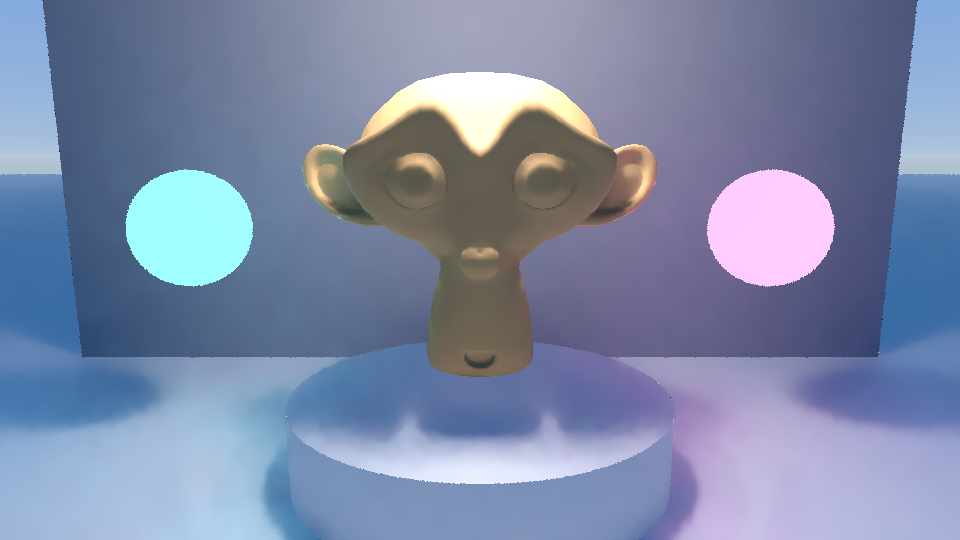
\includegraphics[width=0.78\textwidth]{docs/assets/scene3_canonical_clean.png}
  \caption{Escena 3 (\textit{Hybrid Mesh + SDF}): integración de un volumen SDF tridimensional generado a partir de la malla poligonal Suzanne sobre un pedestal con iluminación indirecta procedente de dos orbes emisivos.}
  \label{fig:escena3_suzanne}
\end{figure}

Con el fin de examinar directamente el interior de las texturas tridimensionales sin depender de los efectos ópticos del trazador de rayos (cumpliendo el objetivo específico OE5), se ha diseñado el \textbf{inspector interactivo de cortes ortogonales bidimensionales} (\textit{2D Orthogonal Slice Inspector}) integrado en el shader \texttt{linear\_to\_srgb.frag}. El inspector permite seccionar el volumen activo a lo largo de cualquiera de los tres planos cartesianos principales ($X/YZ$, $Y/XZ$ o $Z/XY$) en una coordenada normalizada $s \in [0, 1]$, ofreciendo dos modos analíticos de representación:

\begin{enumerate}
  \item \textbf{Modo de isolíneas y clasificación de signo (\textit{SDF Isolines \& Sign}):} Codifica las regiones interiores negativas ($f < 0$) mediante una rampa cromática azul y las regiones exteriores positivas ($f > 0$) mediante una rampa cálida naranja, moduladas por la distancia normalizada $|f| / (0,4\,W)$. Sobre este campo continuo se superponen bandas periódicas de isolíneas oscuras cada $2\,\Delta x_{\text{vóxel}}$ mediante una función de onda triangular suavizada y se resalta la isosuperficie cero ($|f| < 0,9\,\Delta x_{\text{vóxel}}$) con un contorno blanco de alta visibilidad.
  \item \textbf{Modo de mapa de calor de error absoluto (\textit{Absolute Error Heatmap} $|f_{\text{JFA}} - f_{\text{ref}}|$):} Muestrea simultáneamente en la misma coordenada tridimensional $\mathbf{u} \in [0, 1]^3$ el volumen candidato generado por cualquiera de las variantes de JFA y el volumen de referencia exacto \texttt{m\_referenceSdfTexture} (\texttt{ExactBaseline} en \texttt{GL\_R32F}). La discrepancia absoluta $|f_{\text{JFA}}(\mathbf{u}) - f_{\text{ref}}(\mathbf{u})|$ se normaliza respecto a una escala de $2\,\Delta x_{\text{vóxel}}$ y se proyecta sobre una paleta perceptual de cinco nodos (azul oscuro $\to$ púrpura $\to$ rojo $\to$ naranja $\to$ amarillo brillante). Adicionalmente, el contorno cero de la solución de referencia se dibuja en color cian y cualquier vóxel donde exista discrepancia de signo ($(f_{\text{JFA}} < 0) \neq (f_{\text{ref}} < 0)$) se marca con un patrón damero magenta de alerta diagnóstica.
\end{enumerate}

Finalmente, el subsistema de instrumentación y perfilado en GPU combina dos niveles de medición complementarios expuestos en el panel lateral de Dear ImGui (que incluye además un marcador opcional en pantalla de las esquinas 3D del volumen estático en cian y del volumen dinámico en rosa mediante \texttt{volume\_bounds.vert}):

\begin{itemize}
  \item \textbf{Temporización asíncrona por fotograma en anillo (\texttt{FrameGpuQueries}):} Durante el bucle interactivo, un búfer circular de 8 conjuntos de seis marcas de tiempo en hardware (\texttt{glQueryCounter} con \texttt{GL\_TIMESTAMP}) registra sin bloquear la CPU ni vaciar la cola de comandos los instantes de inicio y fin del renderizado, de la actualización del volumen SDF dinámico y del pase de trazado de rayos, reportando en tiempo real \texttt{sdfBuildMs}, \texttt{renderMs} y \texttt{pathTraceMs}.
  \item \textbf{Desglose por etapas del generador y evaluación vóxel a vóxel (\texttt{SdfStats}):} En las generaciones bajo demanda, el módulo \texttt{SdfGenerator} mide mediante consultas \texttt{GL\_TIME\_\allowbreak ELAPSED} el tiempo consumido por la etapa de inicialización de semillas (\texttt{seedGpuMs}), el bucle de propagación JFA (\texttt{floodGpuMs}) y la pasada de signo y finalización (\texttt{finalize\allowbreak GpuMs}), calcula el consumo exacto de VRAM estática y temporal en megabytes, y evalúa en \texttt{computeErrorMetrics} las métricas MAE, RMSE, $E_{\max}$ y el porcentaje de coincidencia de signo sobre la totalidad de los $V^3$ vóxeles.
\end{itemize}

\subsection{Verificación experimental preliminar y validación de regresiones}

Para comprobar la corrección funcional del diseño antes de la batería experimental completa del Capítulo~5, se han ejecutado pruebas numéricas, de rendimiento en GPU y de validación visual sobre los módulos implementados, quedando automatizadas en el ejecutable de pruebas de regresión \texttt{render\_tests} (integrado en CTest). La Tabla~\ref{tab:verificacion_preliminar_pec3} resume los principales resultados cuantitativos verificados en las pruebas de validación del sistema.

\begin{table}[htbp]
  \centering
  \footnotesize
  \caption{Resumen de comprobaciones numéricas y mediciones de validación de los módulos implementados.}
  \label{tab:verificacion_preliminar_pec3}
  \begin{tabularx}{\textwidth}{|>{\bfseries\raggedright\arraybackslash}p{33mm}|>{\raggedright\arraybackslash}p{35mm}|>{\raggedright\arraybackslash}p{35mm}|>{\raggedright\arraybackslash}X|}
    \hline
    \rowcolor{tablegray} Experimento / Prueba & Configuración evaluada & Resultado verificado & Interpretación técnica \\ \hline
    Fidelidad de signo y distancia (\texttt{JfaVoxelShell}) & Suzanne ($968$ tris), variantes $\text{JFA}$, $\text{JFA}+1$ y $1+\text{JFA}$ con votación axial (6 dir.) frente a \texttt{ExactBaseline} & Coincidencia de signo del \textbf{100,0 \%} ($> 99,0$ \% en las 3 variantes); MAE de \textbf{0,68 mm} y RMSE $< 0,02\text{ m}$ & La resolución sub-vóxel combinada con el barrido axial reproduce el signo exacto del ángulo sólido con error sub-milimétrico. \\ \hline
    Cuantización \texttt{GL\_R16F} frente a \texttt{GL\_R32F} & \texttt{ExactBaseline} en $32^3$ ($W = 2,0\text{ m}$) comparando 16 bits frente a 32 bits & Reducción del \textbf{50 \%} en VRAM estática; MAE $< 10^{-4}\text{ m}$ y acuerdo de signo $> 99,9$ \% & El formato de 16 bits (\texttt{R16F}) reduce a la mitad la memoria estática sin degradación métrica apreciable. \\ \hline
    Precisión en escena arquitectónica (\texttt{sponza.glb}) & Crytek Sponza ($262.267$ tris, $W = 30\text{ m}$), \texttt{JfaVoxelShell} ($\text{JFA}+1$, sin signo) frente a referencia & Error máximo en banda de semillas ($d < 1,74\,\Delta x$) $< \textbf{0,002}\,\Delta x_{\text{vóxel}}$; MAE global $< \textbf{0,05}\,\Delta x_{\text{vóxel}}$ & La siembra atómica conserva las distancias exactas punto-triángulo en toda la corteza superficial de Sponza. \\ \hline
    Rendimiento de trazado en Crytek Sponza & Trazado en el atrio interior de Sponza con compensación de $0,55\,\Delta x_{\text{vóxel}}$ y guarda de signo & Tiempo de trazado GPU de \textbf{4,31 ms} a $128^3$ y \textbf{3,70 ms} a $256^3$; \textbf{0,00 ms} de generación en fotogramas en caché & La reducción del inflado superficial y el acotamiento de rayos de sombra mantienen tasas interactivas en recintos cerrados. \\ \hline
    Persistencia del objeto dinámico (\texttt{JfaCameraGBuffer}) & Malla móvil Suzanne en Sponza ($48^3$, $4,0\text{ m}$) con acumulación local en giro de $180^\circ$ y vista opuesta & El MAE superficial ($< 1\text{ vóxel}$) baja de \textbf{0,1465 m} (1 vista) a \textbf{0,0349 m} (2 vistas); $> 98$ \% de cobertura y sombra fuera de cámara & La acumulación de semillas en el marco rígido local reconstruye progresivamente la geometría 3D a partir de vistas parciales. \\ \hline
    Profundidad sub-vóxel y oclusor fino (\texttt{StretchingBox}) & Comparación de profundidad primaria SDF frente a malla rasterizada; espesores de $40\text{ mm}$ a $0,1\text{ mm}$ & Cobertura superficial $> 98$ \% sin huecos y error de profundidad $< 0,25\,\Delta x_{\text{vóxel}}$ en $> 85$ \% de los píxeles visibles & La placa con signo detrás de las semillas de cámara evita fugas de luz incluso en oclusores de $0,1\text{ mm}$ de espesor. \\ \hline
    Estabilidad temporal de SVGF en Sponza & Variación media inter-fotograma en bloques estáticos de $8\times 8$ píxeles con objeto móvil activo & Reducción de la fluctuación temporal de luminancia de \textbf{0,0199} a \textbf{0,0045} ($4,4\times$ más estable) & La reproyección dedicada del objeto móvil evita invalidar el historial temporal de la arquitectura estática. \\ \hline
  \end{tabularx}
\end{table}
